\begin{frame}
	\frametitle{RA en entornos universitarios}
			\block{\it Aprendizaje}
				\begin{itemize}
					\item La RA se encuentra preparada para comenzar a acercarse a las aulas.
					\item Capacidad para generar material didactico y actividades para cualquier disciplina.
					\item Mejorar el aprendizaje.
					\item Experiencias mas ricas e inmersivas.
					\item Cambia la forma en la que adquieren los contenidos de aprendizaje.
				\end{itemize}
			\endblock{}
\end{frame}

%------------------------------------------------------------------

\begin{frame}
	\frametitle{RA en entornos universitarios}
		\block{\it Beneficios principales}
			\begin{itemize}
				\item Aumentar o enriquecer la información de la realidad para hacerla más comprensible al alumno.
			
				\item El uso de una interfaz tangible para la manipulación de objetos, que permite observar un objeto desde diferentes puntos de vista,
				seleccionando, el discente, el momento y posición de observación.
			
				\item Potenciar el aprendizaje ubicuo.
				
				\item Crear escenarios ``artificiales'' seguros para el alumnado
				como pueden ser laboratorios o simuladores. 
			
				\item Enriquecer los materiales impresos para el alumnado con información adicional en diferentes soportes.
				
				\item Facilita la colaboración efectiva y discusión entre el alumnado.
			\end{itemize}
		\endblock{}
\end{frame}


%---------------------------------------------------------------------

\begin{frame}
	\frametitle{RA en entornos universitarios}
		\begin{columns}
			\begin{column}{0.6\textwidth}
				\block{\it Diseño de aplicaciones orientadas a la enseñanza}
				\begin{itemize}
					\item Ser sencillo y robusto.
					\item Permitir que el educador ingrese información de manera simple y efectiva.
					\item Proporcionar al alumno información clara y concisa.
					\item Permitir una fácil interacción entre estudiantes y educadores.
					\item Realizar procedimientos complejos transparentes para los alumnos.
					\item Ser rentable y fácilmente extensible.
				\end{itemize}
				\endblock{}
			\end{column}
			\begin{column}{0.4\textwidth}
				\vfill 
				\begin{center}
					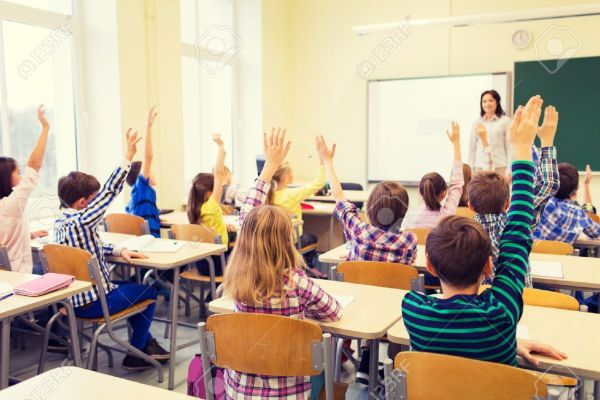
\includegraphics[width=0.9\linewidth]{Images/clase}
				\end{center}
			\end{column}		
		\end{columns}
\end{frame}



\begin{frame}
	\frametitle{RA en entornos universitarios}
		\block{\it Aplicaciones en entornos universitarios}
			\begin{itemize}
				\item Prácticas en laboratorios.
			
				\item Practicas de campo y visitas.
			
				\item Libros y documentos.
				
				\item Aprendizajes experimentales.
			
				\item Información sobre la universidad.
				
			\end{itemize}
		\endblock{}
\end{frame}

\begin{frame}
	\frametitle{RA en entornos universitarios}
		\block{\it Ejemplos de uso de la RA}
		\begin{columns}
			\begin{column}{0.9\textwidth}
				\block{\it Fabricación de un automóvil de carreras}
					\begin{itemize}
						\item El alumnado de la Universidad de Bath está utilizando una nueva herramienta RA que ayudará en la construcción de la carcasa de un automóvil.
						\item  La herramienta ha sido desarrollada por la compañía de tecnología Rocketmakers. 
						\item El vehículo competirá en la competición de Fórmula Estudiantil 2019.
						
					\end{itemize}
				\endblock{}
			\end{column}
		\end{columns}
		\endblock{}
\end{frame}	


\begin{frame}
	\frametitle{RA en entornos universitarios}
	\vfill 
	\begin{center}
		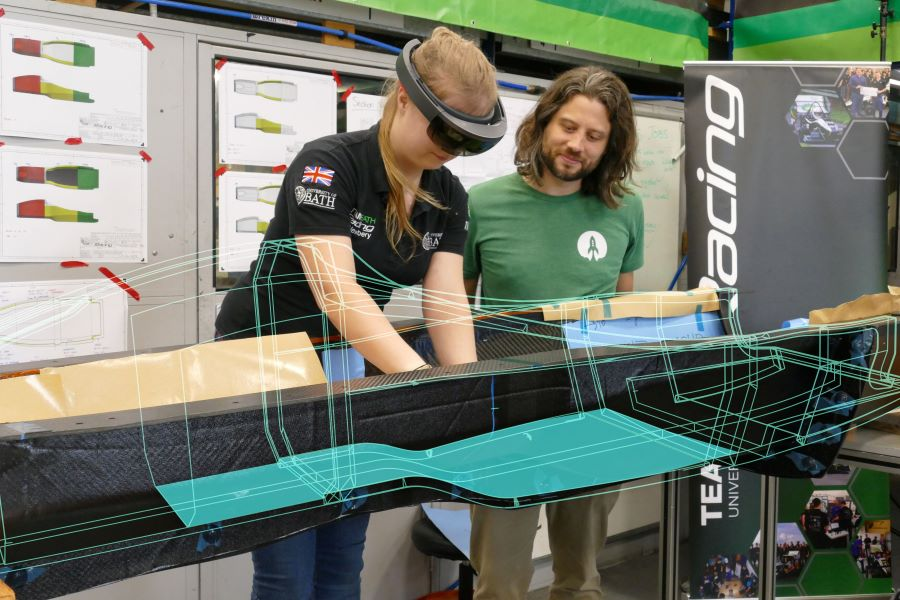
\includegraphics[width=0.8\linewidth]{Images/carARR}
	\end{center}
\end{frame}


\begin{frame}
	\frametitle{RA en entornos universitarios}
	\block{\it Ejemplos de uso de la RA}
	\begin{columns}
		\begin{column}{0.9\textwidth}
			\block{\it Fabricación de un automóvil de carreras}
			\begin{itemize}
				\item Es resultado de un proyecto desarrollado por 
				el \textit{UC Davis W.M. Keck Center for Active Visualization in the Earth Sciences} (KeckCAVES), 
				conjuntamente con el \textit{UC Davis Tahoe Environmental Research Center}, el Lawrence Hall of Science, y el \textit{ECHO Lake Aquarium and Science Center}.
				\item Permite a los usuarios crear modelos de topografía mediante técnicas de RA al dar forma a la arena real. 
					\end{itemize}
				\endblock{}
			\end{column}
		\end{columns}
		\endblock{}
\end{frame}	

\begin{frame}
	\frametitle{RA en entornos universitarios}
	\vfill 
	\begin{center}
		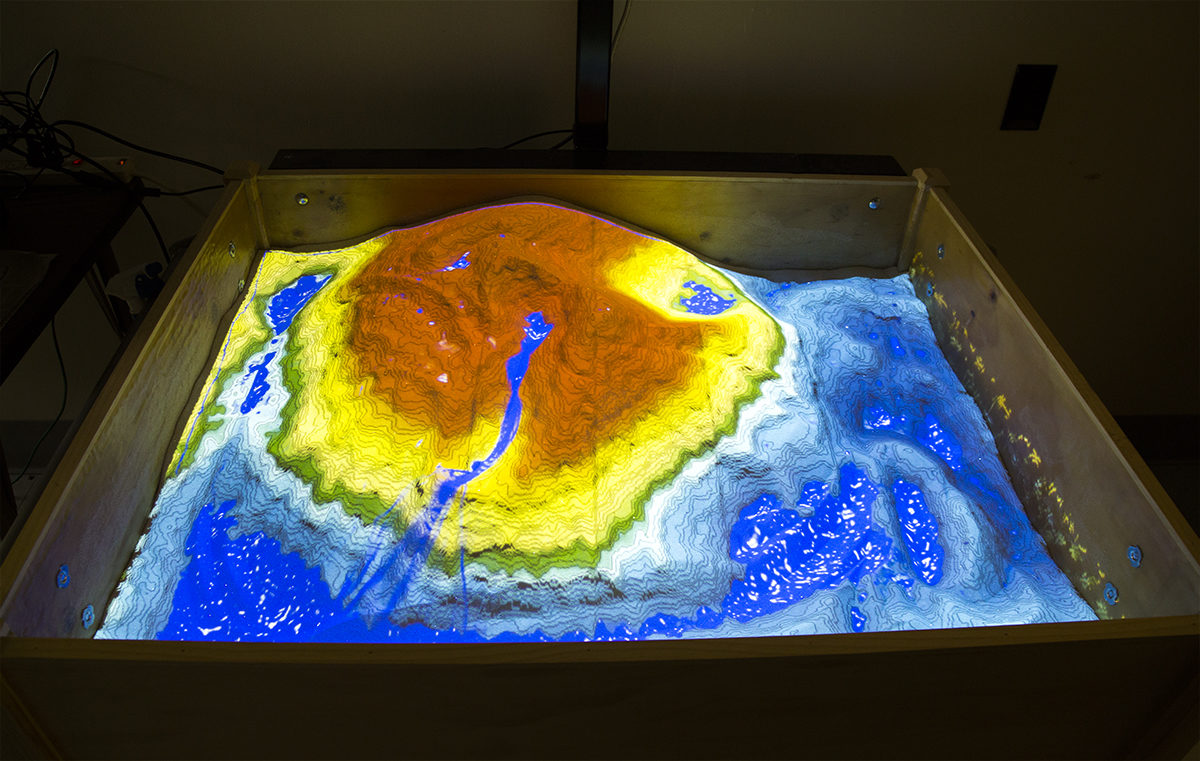
\includegraphics[width=0.8\linewidth]{Images/sandAR}
	\end{center}
\end{frame}


